
\section{How to not optimize the Tabu List}
	In this section I try to understand how different implementations of Tabu list for the Tabu Search method can impact in the quality of the best solution found in a certain amount of time. I also compared the results with the results of the Local Search method.

\subsection{Tabu Search Algorithm}
	I focus my test only on the Tabu Search Best Improvement hence I remove all the others stuff: some switch case and the aspiration criteria.
	The Tabu Search Algorithm is implemented as the Local Search algorithm and it add some operations for managing the tabu list:
	\begin{itemize}
		\item in the choice of a neighbour move it check if that move is into the tabu list;
		\item after the computation of the move it push back the move done and if the tabu list reach the maximum size it pop the front move from the tabu list;
		\item the iteration process is stopped if the time is greater than the maximum time set.
	\end{itemize}
	All the other parts of the algorithm are equal to the Local Search implementation.
	
	
	
	%\begin{itemize}
	%	\item At each iteration if Tabu list size is less of tabu length set the algorithm push back the \verb|TSPMove| into the list;
	%	\item otherwise the algorithm pop the front of the list and
	%\end{itemize}

	\subsection{Implementations variants of Tabu List}
		
		\paragraph{std::List} Initially I implemented the Tabu list mechanism using a standard \verb|List| container. This sequence container allows constant time in the insertion of a single element (\verb|push_back| method) and in the erase of a single element in the front of the list (\verb|pop_front| method)\footnote{from C++11 International Standard §23.3.6.4}.
		The problem with this container is that for checking if a move is a taboo it need $O(n)$ complexity where $n$ is the length of the list.
		
		\paragraph{std::set + std::list} After I detected that with large tabu length the list performs poorly I use a combination of two containers. I use the previously \verb|list| for keeping the order and remove the old move inserted while I use the \verb|set| associative container for get a reduce time of access on my tabu list (now a set). In order to use \verb|set| I encoding a move into a \verb|string|, precisely a concatenation of the two integer \verb|from| and \verb|to|. For example Move of \verb|3| and \verb|7| begin the string \verb|"37"| that I use as key value for the \verb|set|.
		
		\verb|set| container allows insertion  with $N \cdot log (setActualSize + N)$ of complexity, erasing with $log(setActualSize) +  1$ (greater than \verb|List| complexity) but it allows an access with a logarithmic complexity\footnote{C++11 International Standard Table 102 §23.2.4}. 

\subsection{Settings}
\label{subsec:settings}
The following list show the settings for Tabu Search and Local Search:
\begin{itemize}
	\item Best Improvement;
	\item Instance \verb|DS_1120| of 1120 nodes (a restriction due to my time limit);
	\item Maximum computation time 10 seconds;
	\item Four different tabu length values: (the number were chosen keeping in mind the previous report)
	\begin{itemize}
		\item 0;
		\item 20;
		\item 180;
		\item 480.
	\end{itemize}
\end{itemize}

\subsection{Test}
	Since I use the time as stop criteria I decided also to keep in consideration the number of iterations on computation. I consider that more iterations means more probability to find a better value.
	

	
	
	%1
	\paragraph*{}
	In the \textbf{first test} I started the tabu search (settings \ref{subsec:settings}) with \verb|list| and \verb|set+list| with the same initial random solution. The Figure \ref{fig:oneinitrnd} shows that the \verb|set+list| has in all cases a bad performance, instead the \verb|list| goes bad when the list length is large.
	
	This is caused by the fact that the instance \verb|DS_1120| is very large and the convergence on a first local minimum need a lot of iterations (about 1400, result from a Local Search). This could depends on:
	\begin{itemize}
		\item the tabu length, if the length is set to high value the tabu search do diversification;
		\item the time for check if a move is a tabu. For the \verb|set+list| also the time for encoding the move.
	\end{itemize} 
	
	\begin{figure}
		\centering
		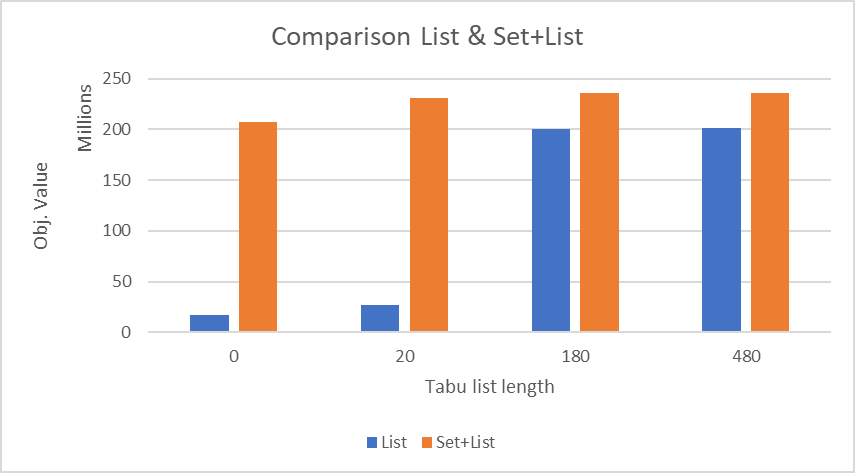
\includegraphics[width=\linewidth]{img/OneInitRnd}
		\caption{Comparison results from list and set+list with search that starts from one random solution.}
		\label{fig:oneinitrnd}
	\end{figure}
	
	
	%2
	\paragraph*{}
	The next test start the tabu search (settings \ref{subsec:settings}) with 8 different initial solution. 10 seconds for each search means a total of 80 seconds for each search execution. In the Table \ref{tab:8initrnd_1} we can see in the column \textbf{Best Value} that \verb|list| found a better solution, unexpectedly the average values for \verb|list| with tabu length 180 and 480 is a lot worse than the average values of \verb|set+list|. The average iterations also indicate that something strange happens with \verb|list|. 
	
	From this strange data a deep inspections on code help me to find a bug in the program. Simply the Tabu Search with \verb|list| executes with the first initial random solution, since the tabu length is big it converges slowly but faster than \verb|set+list| therefore it found a better value than \verb|set+list|. And here the problem comes out: in the next search with another random solution the Tabu list remains the same of the previous search. In this case the converge is even slower cause a lot of move is already tabu and the list is full, that means more time for checking if a move is tabu from the beginning.
	
	In the Table \ref{tab:8initrnd_2} I report the correct data with the bug fixed.
	
	\begin{table}[]
		\centering
		\begin{tabular}{lrrrr}
			\toprule
			\textbf{Data Structure} & \textbf{Length} & \textbf{Avg Value} & \textbf{Best Value} & \textbf{Avg Iterations} \\
			\midrule
			list                    & 0               & 17051200           & 16969100            & 2727                    \\
			& 20              & 26326800           & 25443800            & 825                     \\
			& 180             & 271610000          & 201459000           & 89                      \\
			& 480             & 303803000          & 201459000           & 60                      \\
			\midrule
			set+list                & 0               & 203752000          & 201090000           & 166                     \\
			& 20              & 230667000          & 227666000           & 133                     \\
			& 180             & 241846000          & 234082000           & 120                     \\
			& 480             & 245638000          & 234082000           & 115   \\
			\bottomrule                 
		\end{tabular}
		\caption{Comparison results from list and set+list with search that starts from eight random solution.}
		\label{tab:8initrnd_1}
	\end{table}

	\begin{table}[]
		\centering
		\begin{tabular}{lrrrr}
			\toprule
			\textbf{Solver} & \textbf{Length} & \textbf{Ag Value} & \textbf{Best Value} & \textbf{Avg Iterations} \\
			\toprule
			LS              & -                                   & 17051200                              & 16969100                                & 1388                                        \\
			\midrule
			TS BI list      & 0                                   & 17051200                              & 16969100                                & 2709                                        \\
			& 20                                  & 25677700                              & 24583600                                & 842                                         \\
			& 180                                 & 202994000                             & 200345000                               & 167                                         \\
			& 480                                 & 202713000                             & 200128000                               & 168                                         \\
			\midrule
			TS BI set+list  & 0                                   & 205943000                             & 203128000                               & 163 \\
			& 20                                  & 231721000                             & 228689000                               & 131 \\
			& 180                                 & 236721000                             & 232739000                               & 125  \\
			& 480                                 & 236722000                             & 233591000                               & 125  \\
			\bottomrule
		\end{tabular}
		\caption{Comparison results from LS, TS list and TS set+list with search that starts from eight random solution with the bug fixed.}
		\label{tab:8initrnd_2}
	\end{table}
	

\newpage
		
\subsection{Conclusion}
	Why \verb|set+list| performs so poorly? One fact not take in consideration is the encoding of the \verb|Move| into a string. This operation is very slow with the methods that I used\footnote{Test of different method on different compiler: \\ \href{https://tinodidriksen.com/2010/02/cpp-convert-int-to-string-speed/}{https://tinodidriksen.com/cpp-convert-int-to-string-speed} and also challenges: \\ \href{https://stackoverflow.com/questions/4351371/c-performance-challenge-integer-to-stdstring-conversion}{https://stackoverflow.com/c-performance-challenge-integer-to-stdstring-conversion}.}. 
	Another thing that we need to keep in consideration is that a \verb|set| is a big data structure (a balanced tree) that take about 3 times the memory needed for a simply vector and this means more page faults\footnote{Scott Meyers, Effective STL §3.19.}. This fact maybe justify why the \verb|set+list| performs bad also if tabu length is set to 0, but this fact needs a more deep inspection.
	
	Apart from this stuff about the \verb|set| the main problem on the Tabu Search implemented was the bug where the tabu list was not clear before the start of another search operation. This does not mean that the data collected in the previous report is incorrect, they simply are collected with a special (involuntary) technique where the tabu list was recycled from the previous search at the start of the next search with a different initial random solution. 
	
	In conclusion:
	\begin{itemize}
		\item For small tabu list the standard \verb|list| is more suitable and performs better.
		\item The average of iterations decrease less using a \verb|set+list| than a \verb|list|. In case of the need of a large tabu list, this could be an alternative. In the literature often this is not the case, others container or tricks could performs much better\footnote{hash set is a valid variants of set. Sorted vector often are use as substitute of an associative container.}.
	\end{itemize}
	
